%
% db-binomialverteilung.tex -- Datenblatt der Binomialverteilung
%
% (c) 2015 Prof Dr Andreas Mueller, Hochschule Rapperswil
%
\subsection{Steckbrief}
\begin{center}
\renewcommand{\arraystretch}{1.5}
\begin{tabular}{|l|l|}
\hline
Name&Binomialverteilung\\
\hline
Wahrscheinlichkeit&
\begin{minipage}{3.7in}
\vskip3pt
$\displaystyle P(k)=\binom{n}{k}p^k(1-p)^{n-k}$
\end{minipage}
\\[10pt]
Verteilungsfunktion&
$\displaystyle F(k)=\sum_{i=0}^k\binom{n}{i}p^i(1-p)^{n-i}$
\\[10pt]
Erwartungswert&$\displaystyle np$\\
Varianz&$\displaystyle np(1-p)$\\
\hline
Anwendungen&\begin{minipage}{3.7in}%
\strut
$\bullet$ Anzahl Eintreten eines Bernoulli-Experimentes
\strut
\end{minipage}\\
\hline
\end{tabular}
\end{center}

\subsection{Verteilungsfunktion und Wahrscheinlichkeitsverteilung}
Wahrscheinlichkeitsverteilung und Verteilungsfunktion einer
Binomialverteilung mit $p=0.4$ und $n=10$:
\begin{center}
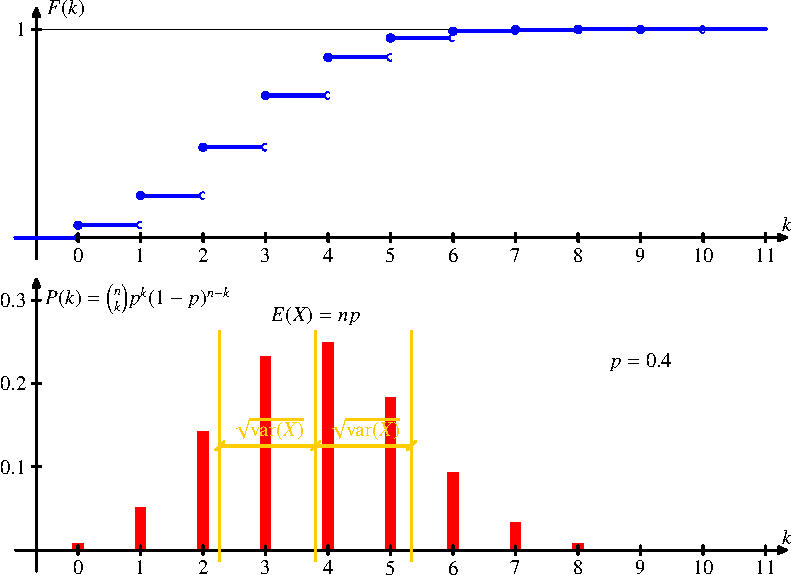
\includegraphics{images/gl-3.pdf}
\end{center}

\subsection{Parameter sch"atzen}
Wir ein Bernoulli-Experiment mit $m$ Wiederholungen $n$ mal wiederholt, erh"alt
man $n$ Werte $k_1,\dots,k_n$.
Die Wahrscheinlichkeit $p$ kann daraus mit Hilfe des Mittelwertes erwartungstreu
gesch"atzt werden:
\[
\hat p(k_1,\dots, k_n)=\frac{k_1+\dots+k_n}{n}.
\]
Als Sch"atzer f"ur den Parameter $m$ liegt das Maximum nahe, da aber
grosse Werte sehr selten sind, ist dieser Sch"atzer von unbrauchbarer
Qualit"at.

